\documentclass[twoside]{book}

% Packages required by doxygen
\usepackage{fixltx2e}
\usepackage{calc}
\usepackage{doxygen}
\usepackage[export]{adjustbox} % also loads graphicx
\usepackage{graphicx}
\usepackage[utf8]{inputenc}
\usepackage{makeidx}
\usepackage{multicol}
\usepackage{multirow}
\PassOptionsToPackage{warn}{textcomp}
\usepackage{textcomp}
\usepackage[nointegrals]{wasysym}
\usepackage[table]{xcolor}

% Font selection
\usepackage[T1]{fontenc}
\usepackage[scaled=.90]{helvet}
\usepackage{courier}
\usepackage{amssymb}
\usepackage{sectsty}
\renewcommand{\familydefault}{\sfdefault}
\allsectionsfont{%
  \fontseries{bc}\selectfont%
  \color{darkgray}%
}
\renewcommand{\DoxyLabelFont}{%
  \fontseries{bc}\selectfont%
  \color{darkgray}%
}
\newcommand{\+}{\discretionary{\mbox{\scriptsize$\hookleftarrow$}}{}{}}

% Page & text layout
\usepackage{geometry}
\geometry{%
  a4paper,%
  top=2.5cm,%
  bottom=2.5cm,%
  left=2.5cm,%
  right=2.5cm%
}
\tolerance=750
\hfuzz=15pt
\hbadness=750
\setlength{\emergencystretch}{15pt}
\setlength{\parindent}{0cm}
\setlength{\parskip}{3ex plus 2ex minus 2ex}
\makeatletter
\renewcommand{\paragraph}{%
  \@startsection{paragraph}{4}{0ex}{-1.0ex}{1.0ex}{%
    \normalfont\normalsize\bfseries\SS@parafont%
  }%
}
\renewcommand{\subparagraph}{%
  \@startsection{subparagraph}{5}{0ex}{-1.0ex}{1.0ex}{%
    \normalfont\normalsize\bfseries\SS@subparafont%
  }%
}
\makeatother

% Headers & footers
\usepackage{fancyhdr}
\pagestyle{fancyplain}
\fancyhead[LE]{\fancyplain{}{\bfseries\thepage}}
\fancyhead[CE]{\fancyplain{}{}}
\fancyhead[RE]{\fancyplain{}{\bfseries\leftmark}}
\fancyhead[LO]{\fancyplain{}{\bfseries\rightmark}}
\fancyhead[CO]{\fancyplain{}{}}
\fancyhead[RO]{\fancyplain{}{\bfseries\thepage}}
\fancyfoot[LE]{\fancyplain{}{}}
\fancyfoot[CE]{\fancyplain{}{}}
\fancyfoot[RE]{\fancyplain{}{\bfseries\scriptsize Generated by Doxygen }}
\fancyfoot[LO]{\fancyplain{}{\bfseries\scriptsize Generated by Doxygen }}
\fancyfoot[CO]{\fancyplain{}{}}
\fancyfoot[RO]{\fancyplain{}{}}
\renewcommand{\footrulewidth}{0.4pt}
\renewcommand{\chaptermark}[1]{%
  \markboth{#1}{}%
}
\renewcommand{\sectionmark}[1]{%
  \markright{\thesection\ #1}%
}

% Indices & bibliography
\usepackage{natbib}
\usepackage[titles]{tocloft}
\setcounter{tocdepth}{3}
\setcounter{secnumdepth}{5}
\makeindex

% Hyperlinks (required, but should be loaded last)
\usepackage{ifpdf}
\ifpdf
  \usepackage[pdftex,pagebackref=true]{hyperref}
\else
  \usepackage[ps2pdf,pagebackref=true]{hyperref}
\fi
\hypersetup{%
  colorlinks=true,%
  linkcolor=blue,%
  citecolor=blue,%
  unicode%
}

% Custom commands
\newcommand{\clearemptydoublepage}{%
  \newpage{\pagestyle{empty}\cleardoublepage}%
}

\usepackage{caption}
\captionsetup{labelsep=space,justification=centering,font={bf},singlelinecheck=off,skip=4pt,position=top}

%===== C O N T E N T S =====

\begin{document}

% Titlepage & ToC
\hypersetup{pageanchor=false,
             bookmarksnumbered=true,
             pdfencoding=unicode
            }
\pagenumbering{alph}
\begin{titlepage}
\vspace*{7cm}
\begin{center}%
{\Large Lattice Q\+CD for Novices\+: 1D Montecarlo Path Integration }\\
\vspace*{1cm}
{\large Generated by Doxygen 1.8.13}\\
\end{center}
\end{titlepage}
\clearemptydoublepage
\pagenumbering{roman}
\tableofcontents
\clearemptydoublepage
\pagenumbering{arabic}
\hypersetup{pageanchor=true}

%--- Begin generated contents ---
\chapter{Main Page}
\label{index}\hypertarget{index}{}\hypertarget{index_intro}{}\section{Introduction}\label{index_intro}
The purpose of this code is to reproduce the second excercise in Lepage\textquotesingle{}s article \char`\"{}\+Lattice Q\+C\+D for Novices\char`\"{}. A 1D quantum system is path integrated using the Montecarlo algorithm in order to provide estimates of first excited state energy gap.

The source code is composed of five files\+: \hyperlink{SETTINGS_8h}{S\+E\+T\+T\+I\+N\+G\+S.\+h}, \hyperlink{CUSTOM_8h}{C\+U\+S\+T\+O\+M.\+h}, \hyperlink{Metropolis_8h}{Metropolis.\+h}, Metropolis.\+cpp and \hyperlink{1D__path__integral_8cpp}{1\+D\+\_\+path\+\_\+integral.\+cpp} ~\newline
The plot routines are given in two versions\+: \hyperlink{plot__macro_8cpp}{plot\+\_\+macro.\+cpp} and \hyperlink{plot__macro_8py}{plot\+\_\+macro.\+py}.\hypertarget{index_reqs}{}\section{Requirements}\label{index_reqs}

\begin{DoxyItemize}
\item To compute the results\+: g++ compiler
\item To plot the results\+: either R\+O\+OT (download at \href{https://root.cern/install/}{\tt https\+://root.\+cern/install/}) or a working Python installation.
\end{DoxyItemize}\hypertarget{index_build}{}\section{How to Build and Run}\label{index_build}

\begin{DoxyItemize}
\item It is suggested to create a copy of the 1\+D\+\_\+path\+\_\+integral directory, so as to keep the sequence of experiments separated
\item Provide the system definition and the required observables in \hyperlink{CUSTOM_8h}{C\+U\+S\+T\+O\+M.\+h}
\item Check and set the parameters in \hyperlink{SETTINGS_8h}{S\+E\+T\+T\+I\+N\+G\+S.\+h}
\item Execute the script B\+U\+I\+L\+D.\+sh ~\newline
 \$ ./\+B\+U\+I\+LD.sh
\item Run the executable ~\newline
 \$ ./executable
\item Check the output file
\end{DoxyItemize}\hypertarget{index_plot}{}\section{How to plot}\label{index_plot}

\begin{DoxyItemize}
\item Using R\+O\+OT ~\newline
 \$ root \hyperlink{plot__macro_8cpp}{plot\+\_\+macro.\+cpp}
\item Using Python ~\newline
 \$ python \hyperlink{plot__macro_8py}{plot\+\_\+macro.\+py}
\end{DoxyItemize}\hypertarget{index_clean}{}\section{How to Clean}\label{index_clean}

\begin{DoxyItemize}
\item Remove all the output ~\newline
 \$ ./\+C\+L\+E\+AN.sh
\item N\+O\+TE\+: plots and output files are deleted in this procedure 
\end{DoxyItemize}
\chapter{Class Index}
\section{Class List}
Here are the classes, structs, unions and interfaces with brief descriptions\+:\begin{DoxyCompactList}
\item\contentsline{section}{\hyperlink{classMetropolis}{Metropolis} }{\pageref{classMetropolis}}{}
\end{DoxyCompactList}

\chapter{File Index}
\section{File List}
Here is a list of all documented files with brief descriptions\+:\begin{DoxyCompactList}
\item\contentsline{section}{\hyperlink{1D__path__integral_8cpp}{1\+D\+\_\+path\+\_\+integral.\+cpp} \\*Code to path integrate a 1D quantum system with Montecarlo method }{\pageref{1D__path__integral_8cpp}}{}
\item\contentsline{section}{\hyperlink{CUSTOM_8h}{C\+U\+S\+T\+O\+M.\+h} \\*Header file to define the action of the system and the observables to be computed }{\pageref{CUSTOM_8h}}{}
\item\contentsline{section}{\hyperlink{Metropolis_8h}{Metropolis.\+h} \\*Header file for the definition of the class \hyperlink{classMetropolis}{Metropolis} }{\pageref{Metropolis_8h}}{}
\item\contentsline{section}{\hyperlink{plot__macro_8cpp}{plot\+\_\+macro.\+cpp} \\*R\+O\+OT macro to generate a plot from the \hyperlink{1D__path__integral_8cpp}{1\+D\+\_\+path\+\_\+integral.\+cpp} output }{\pageref{plot__macro_8cpp}}{}
\item\contentsline{section}{\hyperlink{plot__macro_8py}{plot\+\_\+macro.\+py} \\*Python code to generate a plot from the \hyperlink{1D__path__integral_8cpp}{1\+D\+\_\+path\+\_\+integral.\+cpp} output }{\pageref{plot__macro_8py}}{}
\item\contentsline{section}{\hyperlink{SETTINGS_8h}{S\+E\+T\+T\+I\+N\+G\+S.\+h} \\*Header file to set the adjustable parameters of the system }{\pageref{SETTINGS_8h}}{}
\end{DoxyCompactList}

\chapter{Class Documentation}
\hypertarget{classMetropolis}{}\section{Metropolis Class Reference}
\label{classMetropolis}\index{Metropolis@{Metropolis}}


{\ttfamily \#include $<$Metropolis.\+h$>$}



Collaboration diagram for Metropolis\+:
\nopagebreak
\begin{figure}[H]
\begin{center}
\leavevmode
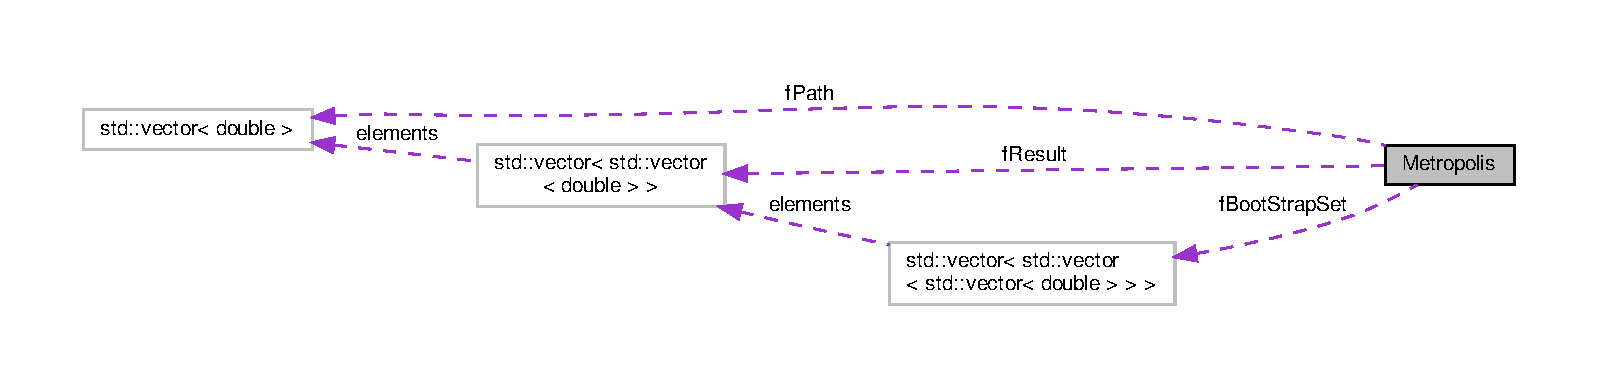
\includegraphics[width=350pt]{classMetropolis__coll__graph}
\end{center}
\end{figure}
\subsection*{Public Member Functions}
\begin{DoxyCompactItemize}
\item 
\hyperlink{classMetropolis_ac702bd026368a444886580d372a99018}{Metropolis} (int \hyperlink{SETTINGS_8h_a7722c8ecbb62d99aee7ce68b1752f337}{N}, int N\+\_\+corr, int N\+\_\+cf, int N\+\_\+bootstraps, double \hyperlink{SETTINGS_8h_a4904cc82627458fdf6672ccc0b2802c7}{epsilon}, double \hyperlink{SETTINGS_8h_a1031d0e0a97a340abfe0a6ab9e831045}{a})
\item 
\mbox{\Hypertarget{classMetropolis_aeeea5bedaa30567a6d1a26e829a40cad}\label{classMetropolis_aeeea5bedaa30567a6d1a26e829a40cad}} 
\hyperlink{classMetropolis_aeeea5bedaa30567a6d1a26e829a40cad}{$\sim$\+Metropolis} ()
\begin{DoxyCompactList}\small\item\em \hyperlink{classMetropolis}{Metropolis} destructor. \end{DoxyCompactList}\item 
int \hyperlink{classMetropolis_acaa8e2e9e8e13f0333f2fc0dd17ab135}{GetN} () const
\item 
int \hyperlink{classMetropolis_abd453b3613ebecb226c0e8ad07ac26cf}{Get\+Ncorr} () const
\item 
int \hyperlink{classMetropolis_a1ac082e2dbbadb602fb30cb15d945a14}{Get\+Ncf} () const
\item 
double \hyperlink{classMetropolis_abc94add65bfe37e91150b68ddbabfc55}{Get\+Epsilon} () const
\item 
double \hyperlink{classMetropolis_a5fef962bc6deca9c57dc377ef5000432}{GetA} () const
\item 
std\+::vector$<$ double $>$ \hyperlink{classMetropolis_af58aa9fe0d0155534a9b1ad90fabbb9e}{Get\+Current\+Path} () const
\item 
std\+::vector$<$ std\+::vector$<$ double $>$ $>$ \hyperlink{classMetropolis_ab8f12fd15c8f3b44bf7384918f9427c8}{Get\+Current\+Result} () const
\item 
\mbox{\Hypertarget{classMetropolis_ac14a16ae31144d70014ae8023c5a9001}\label{classMetropolis_ac14a16ae31144d70014ae8023c5a9001}} 
void \hyperlink{classMetropolis_ac14a16ae31144d70014ae8023c5a9001}{Print\+Current\+Path} () const
\begin{DoxyCompactList}\small\item\em Print the current path configuration on standard output. \end{DoxyCompactList}\item 
double \hyperlink{classMetropolis_afb509c80a84817bf9b4ff183e02a44cb}{S} (int j) const
\item 
double \hyperlink{classMetropolis_a79beaf1cf27f27cd43b7d1d03289d301}{Update\+Current\+Path} ()
\item 
void \hyperlink{classMetropolis_adaa45159158dd78986b830930c3b0b9e}{Run\+Metropolis} ()
\item 
void \hyperlink{classMetropolis_ac0891905d6107b4b442455579314279c}{Boot\+Strap} ()
\item 
double \hyperlink{classMetropolis_adf0ef3e12d4ce4185d3a536649de5cee}{Evaluate\+Gamma} (const std\+::vector$<$ double $>$ \&path, int n) const
\item 
double \hyperlink{classMetropolis_aa0e41567dcbb736f1bcc4a09dbb5f6fb}{Evaluate\+Propagator} (const std\+::vector$<$ double $>$ \&path, int n) const
\item 
void \hyperlink{classMetropolis_aa8fc09048815c71e0a94f314afd631cc}{Compute\+Gamma\+Estimators} ()
\item 
void \hyperlink{classMetropolis_a197d44f9109ce75781a70441f1d0b2b2}{Compute\+Energy\+Estimators} (std\+::string filename)
\item 
void \hyperlink{classMetropolis_aa733da324aa14e6c2fcf9c75f5643cbe}{Compute\+Binned\+Energy\+Estimators} (int bin\+\_\+width, std\+::string \hyperlink{SETTINGS_8h_a4bfaa4b497cb5e62d0cfc56f5ce8cfc9}{output\+\_\+name}) const
\end{DoxyCompactItemize}
\subsection*{Private Member Functions}
\begin{DoxyCompactItemize}
\item 
void \hyperlink{classMetropolis_abfc33a0d7604c24e0337e8a16fa60971}{Print\+Status} (int index, int N\+\_\+max) const
\end{DoxyCompactItemize}
\subsection*{Private Attributes}
\begin{DoxyCompactItemize}
\item 
\mbox{\Hypertarget{classMetropolis_a015b0ab958c4e338d1cdaf19851297a5}\label{classMetropolis_a015b0ab958c4e338d1cdaf19851297a5}} 
const int \hyperlink{classMetropolis_a015b0ab958c4e338d1cdaf19851297a5}{fN}
\begin{DoxyCompactList}\small\item\em Number of grid points for the discretized trajectory. \end{DoxyCompactList}\item 
\mbox{\Hypertarget{classMetropolis_a631ff9cb571718a1b7db5ef9efdaff87}\label{classMetropolis_a631ff9cb571718a1b7db5ef9efdaff87}} 
const int \hyperlink{classMetropolis_a631ff9cb571718a1b7db5ef9efdaff87}{f\+Ncorr}
\begin{DoxyCompactList}\small\item\em Number of correlated configurations to skip before next acquisition. \end{DoxyCompactList}\item 
\mbox{\Hypertarget{classMetropolis_a6607146aa35a49c876ee32b7523c2faf}\label{classMetropolis_a6607146aa35a49c876ee32b7523c2faf}} 
const int \hyperlink{classMetropolis_a6607146aa35a49c876ee32b7523c2faf}{f\+Ncf}
\begin{DoxyCompactList}\small\item\em Number of configurations to sample. \end{DoxyCompactList}\item 
\mbox{\Hypertarget{classMetropolis_a3b599c6ae2343478cb6aaf9a6f579785}\label{classMetropolis_a3b599c6ae2343478cb6aaf9a6f579785}} 
const int \hyperlink{classMetropolis_a3b599c6ae2343478cb6aaf9a6f579785}{f\+N\+Boot\+Straps}
\begin{DoxyCompactList}\small\item\em Number of statistical bootstraps to perform. \end{DoxyCompactList}\item 
\mbox{\Hypertarget{classMetropolis_aaf81aa8fa54ef1e96b9fce05081a4a9a}\label{classMetropolis_aaf81aa8fa54ef1e96b9fce05081a4a9a}} 
const double \hyperlink{classMetropolis_aaf81aa8fa54ef1e96b9fce05081a4a9a}{f\+Epsilon}
\begin{DoxyCompactList}\small\item\em Typical magnitude of the path update. \end{DoxyCompactList}\item 
\mbox{\Hypertarget{classMetropolis_ad9ff6ca323cf287905aaf3c5e7f25cad}\label{classMetropolis_ad9ff6ca323cf287905aaf3c5e7f25cad}} 
const double \hyperlink{classMetropolis_ad9ff6ca323cf287905aaf3c5e7f25cad}{fA}
\begin{DoxyCompactList}\small\item\em Time step in the time discretization. \end{DoxyCompactList}\item 
\mbox{\Hypertarget{classMetropolis_aaed710e91d19ab1a0356c864d105efbe}\label{classMetropolis_aaed710e91d19ab1a0356c864d105efbe}} 
std\+::vector$<$ double $>$ \hyperlink{classMetropolis_aaed710e91d19ab1a0356c864d105efbe}{f\+Path}
\begin{DoxyCompactList}\small\item\em Vector containing the current path configuration\+: it is initialized to zero. \end{DoxyCompactList}\item 
\mbox{\Hypertarget{classMetropolis_aaf8912c959d11c683d7222fbb0e0ec39}\label{classMetropolis_aaf8912c959d11c683d7222fbb0e0ec39}} 
std\+::vector$<$ std\+::vector$<$ double $>$ $>$ \hyperlink{classMetropolis_aaf8912c959d11c683d7222fbb0e0ec39}{f\+Result}
\begin{DoxyCompactList}\small\item\em Matrix containing the sampled configurations. \end{DoxyCompactList}\item 
std\+::vector$<$ std\+::vector$<$ std\+::vector$<$ double $>$ $>$ $>$ \hyperlink{classMetropolis_ae7950341ed835f9ec689b46b2a913bed}{f\+Boot\+Strap\+Set}
\end{DoxyCompactItemize}


\subsection{Detailed Description}
\hyperlink{classMetropolis}{Metropolis} class

Class representing a 1D quantum physical system whose evolution can be computed by path integration using the \hyperlink{classMetropolis}{Metropolis} algorithm. 

\subsection{Constructor \& Destructor Documentation}
\mbox{\Hypertarget{classMetropolis_ac702bd026368a444886580d372a99018}\label{classMetropolis_ac702bd026368a444886580d372a99018}} 
\index{Metropolis@{Metropolis}!Metropolis@{Metropolis}}
\index{Metropolis@{Metropolis}!Metropolis@{Metropolis}}
\subsubsection{\texorpdfstring{Metropolis()}{Metropolis()}}
{\footnotesize\ttfamily Metropolis\+::\+Metropolis (\begin{DoxyParamCaption}\item[{int}]{N,  }\item[{int}]{N\+\_\+corr,  }\item[{int}]{N\+\_\+cf,  }\item[{int}]{N\+\_\+bootstraps,  }\item[{double}]{epsilon,  }\item[{double}]{a }\end{DoxyParamCaption})}

\hyperlink{classMetropolis}{Metropolis} constructor

Constructor of the \hyperlink{classMetropolis}{Metropolis} class 
\begin{DoxyParams}{Parameters}
{\em N} & number of grid points for the discretized trajectory \\
\hline
{\em N\+\_\+corr} & number of correlated configurations to skip before next acquisition \\
\hline
{\em N\+\_\+cf} & number of configurations to sample \\
\hline
{\em N\+\_\+bootstraps} & number of statistical bootstraps to perform when Boot\+Strap function is called \\
\hline
{\em epsilon} & typical magnitude of the path update \\
\hline
{\em a} & time step in the time discretization \\
\hline
\end{DoxyParams}


\subsection{Member Function Documentation}
\mbox{\Hypertarget{classMetropolis_ac0891905d6107b4b442455579314279c}\label{classMetropolis_ac0891905d6107b4b442455579314279c}} 
\index{Metropolis@{Metropolis}!Boot\+Strap@{Boot\+Strap}}
\index{Boot\+Strap@{Boot\+Strap}!Metropolis@{Metropolis}}
\subsubsection{\texorpdfstring{Boot\+Strap()}{BootStrap()}}
{\footnotesize\ttfamily void Metropolis\+::\+Boot\+Strap (\begin{DoxyParamCaption}{ }\end{DoxyParamCaption})}

Statistical bootstrap

Perform a statistical bootstrap to obtain the N\+Boot\+Straps copies of the sampled configurations. \mbox{\Hypertarget{classMetropolis_aa733da324aa14e6c2fcf9c75f5643cbe}\label{classMetropolis_aa733da324aa14e6c2fcf9c75f5643cbe}} 
\index{Metropolis@{Metropolis}!Compute\+Binned\+Energy\+Estimators@{Compute\+Binned\+Energy\+Estimators}}
\index{Compute\+Binned\+Energy\+Estimators@{Compute\+Binned\+Energy\+Estimators}!Metropolis@{Metropolis}}
\subsubsection{\texorpdfstring{Compute\+Binned\+Energy\+Estimators()}{ComputeBinnedEnergyEstimators()}}
{\footnotesize\ttfamily void Metropolis\+::\+Compute\+Binned\+Energy\+Estimators (\begin{DoxyParamCaption}\item[{int}]{bin\+\_\+width,  }\item[{std\+::string}]{output\+\_\+name }\end{DoxyParamCaption}) const}

Compute binned energy estimators

Compute and print on file the Montecarlo estimators for the energy gap between ground state and first excitated state. Uncertainty is estimated by building a set of bootstrap copies of the Montecarlo ensemble and evaluating the associated standard deviation. In this method, before the bootstrap ensemble is built, a binning procedure is performed on the set of Montecarlo configurations. 
\begin{DoxyParams}{Parameters}
{\em bin\+\_\+width} & integer bin width, i.\+e. number of configurations to average to build a bin \\
\hline
{\em output\+\_\+name} & name of the output file \\
\hline
\end{DoxyParams}
\mbox{\Hypertarget{classMetropolis_a197d44f9109ce75781a70441f1d0b2b2}\label{classMetropolis_a197d44f9109ce75781a70441f1d0b2b2}} 
\index{Metropolis@{Metropolis}!Compute\+Energy\+Estimators@{Compute\+Energy\+Estimators}}
\index{Compute\+Energy\+Estimators@{Compute\+Energy\+Estimators}!Metropolis@{Metropolis}}
\subsubsection{\texorpdfstring{Compute\+Energy\+Estimators()}{ComputeEnergyEstimators()}}
{\footnotesize\ttfamily void Metropolis\+::\+Compute\+Energy\+Estimators (\begin{DoxyParamCaption}\item[{std\+::string}]{filename }\end{DoxyParamCaption})}

Compute energy estimators

Compute and print on file the Montecarlo estimators for the energy gap between ground state and first excitated state. Uncertainty is estimated by building a set of bootstrap copies of the Montecarlo ensemble and evaluating the associated standard deviation. 
\begin{DoxyParams}{Parameters}
{\em filename} & name of the output file \\
\hline
\end{DoxyParams}
\mbox{\Hypertarget{classMetropolis_aa8fc09048815c71e0a94f314afd631cc}\label{classMetropolis_aa8fc09048815c71e0a94f314afd631cc}} 
\index{Metropolis@{Metropolis}!Compute\+Gamma\+Estimators@{Compute\+Gamma\+Estimators}}
\index{Compute\+Gamma\+Estimators@{Compute\+Gamma\+Estimators}!Metropolis@{Metropolis}}
\subsubsection{\texorpdfstring{Compute\+Gamma\+Estimators()}{ComputeGammaEstimators()}}
{\footnotesize\ttfamily void Metropolis\+::\+Compute\+Gamma\+Estimators (\begin{DoxyParamCaption}{ }\end{DoxyParamCaption})}

Compute gamma estimators

Compute and print Montecarlo estimators (expectation value and 1-\/sigma uncertainty) for the observable defined in \hyperlink{classMetropolis_adf0ef3e12d4ce4185d3a536649de5cee}{Metropolis\+::\+Evaluate\+Gamma}. \mbox{\Hypertarget{classMetropolis_adf0ef3e12d4ce4185d3a536649de5cee}\label{classMetropolis_adf0ef3e12d4ce4185d3a536649de5cee}} 
\index{Metropolis@{Metropolis}!Evaluate\+Gamma@{Evaluate\+Gamma}}
\index{Evaluate\+Gamma@{Evaluate\+Gamma}!Metropolis@{Metropolis}}
\subsubsection{\texorpdfstring{Evaluate\+Gamma()}{EvaluateGamma()}}
{\footnotesize\ttfamily double Metropolis\+::\+Evaluate\+Gamma (\begin{DoxyParamCaption}\item[{const std\+::vector$<$ double $>$ \&}]{path,  }\item[{int}]{n }\end{DoxyParamCaption}) const}

Evaluate observable gamma

Define and evaluate the observable gamma whose expectation value is computed in Metropolis\+::\+Compute\+Estimators. Implementation is in the file \hyperlink{CUSTOM_8h}{C\+U\+S\+T\+O\+M.\+h}, which allows for user modification. 
\begin{DoxyParams}{Parameters}
{\em path} & path configuration over which the observable is defined \\
\hline
{\em n} & if the observable depends on time, n is the index corresponding to time t=na, where a is the time step. \\
\hline
\end{DoxyParams}
\mbox{\Hypertarget{classMetropolis_aa0e41567dcbb736f1bcc4a09dbb5f6fb}\label{classMetropolis_aa0e41567dcbb736f1bcc4a09dbb5f6fb}} 
\index{Metropolis@{Metropolis}!Evaluate\+Propagator@{Evaluate\+Propagator}}
\index{Evaluate\+Propagator@{Evaluate\+Propagator}!Metropolis@{Metropolis}}
\subsubsection{\texorpdfstring{Evaluate\+Propagator()}{EvaluatePropagator()}}
{\footnotesize\ttfamily double Metropolis\+::\+Evaluate\+Propagator (\begin{DoxyParamCaption}\item[{const std\+::vector$<$ double $>$ \&}]{path,  }\item[{int}]{n }\end{DoxyParamCaption}) const}

Evaluate propagator

Define and evaluate the propagator whose expectation value is computed in \hyperlink{classMetropolis_a197d44f9109ce75781a70441f1d0b2b2}{Metropolis\+::\+Compute\+Energy\+Estimators}. 
\begin{DoxyParams}{Parameters}
{\em path} & path configuration over which the propagator is computed \\
\hline
{\em n} & integer index corresponding to time t=na, where a is the time step. \\
\hline
\end{DoxyParams}
\mbox{\Hypertarget{classMetropolis_a5fef962bc6deca9c57dc377ef5000432}\label{classMetropolis_a5fef962bc6deca9c57dc377ef5000432}} 
\index{Metropolis@{Metropolis}!GetA@{GetA}}
\index{GetA@{GetA}!Metropolis@{Metropolis}}
\subsubsection{\texorpdfstring{Get\+A()}{GetA()}}
{\footnotesize\ttfamily double Metropolis\+::\+GetA (\begin{DoxyParamCaption}{ }\end{DoxyParamCaption}) const}

\begin{DoxyReturn}{Returns}
a, time step in the time discretization 
\end{DoxyReturn}
\mbox{\Hypertarget{classMetropolis_af58aa9fe0d0155534a9b1ad90fabbb9e}\label{classMetropolis_af58aa9fe0d0155534a9b1ad90fabbb9e}} 
\index{Metropolis@{Metropolis}!Get\+Current\+Path@{Get\+Current\+Path}}
\index{Get\+Current\+Path@{Get\+Current\+Path}!Metropolis@{Metropolis}}
\subsubsection{\texorpdfstring{Get\+Current\+Path()}{GetCurrentPath()}}
{\footnotesize\ttfamily std\+::vector$<$double$>$ Metropolis\+::\+Get\+Current\+Path (\begin{DoxyParamCaption}{ }\end{DoxyParamCaption}) const}

\begin{DoxyReturn}{Returns}
current path configuration, as stored in the private attribute f\+Path 
\end{DoxyReturn}
\mbox{\Hypertarget{classMetropolis_ab8f12fd15c8f3b44bf7384918f9427c8}\label{classMetropolis_ab8f12fd15c8f3b44bf7384918f9427c8}} 
\index{Metropolis@{Metropolis}!Get\+Current\+Result@{Get\+Current\+Result}}
\index{Get\+Current\+Result@{Get\+Current\+Result}!Metropolis@{Metropolis}}
\subsubsection{\texorpdfstring{Get\+Current\+Result()}{GetCurrentResult()}}
{\footnotesize\ttfamily std\+::vector$<$std\+::vector$<$double$>$ $>$ Metropolis\+::\+Get\+Current\+Result (\begin{DoxyParamCaption}{ }\end{DoxyParamCaption}) const}

\begin{DoxyReturn}{Returns}
set of sampled Montecarlo path configurations 
\end{DoxyReturn}
\mbox{\Hypertarget{classMetropolis_abc94add65bfe37e91150b68ddbabfc55}\label{classMetropolis_abc94add65bfe37e91150b68ddbabfc55}} 
\index{Metropolis@{Metropolis}!Get\+Epsilon@{Get\+Epsilon}}
\index{Get\+Epsilon@{Get\+Epsilon}!Metropolis@{Metropolis}}
\subsubsection{\texorpdfstring{Get\+Epsilon()}{GetEpsilon()}}
{\footnotesize\ttfamily double Metropolis\+::\+Get\+Epsilon (\begin{DoxyParamCaption}{ }\end{DoxyParamCaption}) const}

\begin{DoxyReturn}{Returns}
epsilon, typical magnitude of the path update 
\end{DoxyReturn}
\mbox{\Hypertarget{classMetropolis_acaa8e2e9e8e13f0333f2fc0dd17ab135}\label{classMetropolis_acaa8e2e9e8e13f0333f2fc0dd17ab135}} 
\index{Metropolis@{Metropolis}!GetN@{GetN}}
\index{GetN@{GetN}!Metropolis@{Metropolis}}
\subsubsection{\texorpdfstring{Get\+N()}{GetN()}}
{\footnotesize\ttfamily int Metropolis\+::\+GetN (\begin{DoxyParamCaption}{ }\end{DoxyParamCaption}) const}

\begin{DoxyReturn}{Returns}
N, number of grid points for the discretized trajectory 
\end{DoxyReturn}
\mbox{\Hypertarget{classMetropolis_a1ac082e2dbbadb602fb30cb15d945a14}\label{classMetropolis_a1ac082e2dbbadb602fb30cb15d945a14}} 
\index{Metropolis@{Metropolis}!Get\+Ncf@{Get\+Ncf}}
\index{Get\+Ncf@{Get\+Ncf}!Metropolis@{Metropolis}}
\subsubsection{\texorpdfstring{Get\+Ncf()}{GetNcf()}}
{\footnotesize\ttfamily int Metropolis\+::\+Get\+Ncf (\begin{DoxyParamCaption}{ }\end{DoxyParamCaption}) const}

\begin{DoxyReturn}{Returns}
Ncf, number of configurations to sample 
\end{DoxyReturn}
\mbox{\Hypertarget{classMetropolis_abd453b3613ebecb226c0e8ad07ac26cf}\label{classMetropolis_abd453b3613ebecb226c0e8ad07ac26cf}} 
\index{Metropolis@{Metropolis}!Get\+Ncorr@{Get\+Ncorr}}
\index{Get\+Ncorr@{Get\+Ncorr}!Metropolis@{Metropolis}}
\subsubsection{\texorpdfstring{Get\+Ncorr()}{GetNcorr()}}
{\footnotesize\ttfamily int Metropolis\+::\+Get\+Ncorr (\begin{DoxyParamCaption}{ }\end{DoxyParamCaption}) const}

\begin{DoxyReturn}{Returns}
Ncorr, number of correlated configurations to skip before next acquisition 
\end{DoxyReturn}
\mbox{\Hypertarget{classMetropolis_abfc33a0d7604c24e0337e8a16fa60971}\label{classMetropolis_abfc33a0d7604c24e0337e8a16fa60971}} 
\index{Metropolis@{Metropolis}!Print\+Status@{Print\+Status}}
\index{Print\+Status@{Print\+Status}!Metropolis@{Metropolis}}
\subsubsection{\texorpdfstring{Print\+Status()}{PrintStatus()}}
{\footnotesize\ttfamily void Metropolis\+::\+Print\+Status (\begin{DoxyParamCaption}\item[{int}]{index,  }\item[{int}]{N\+\_\+max }\end{DoxyParamCaption}) const\hspace{0.3cm}{\ttfamily [private]}}

Method to plot the status during execution


\begin{DoxyParams}{Parameters}
{\em index} & index of the current step inside the loop \\
\hline
{\em N\+\_\+max} & maximum index, corresponding to the loop ending \\
\hline
\end{DoxyParams}
\mbox{\Hypertarget{classMetropolis_adaa45159158dd78986b830930c3b0b9e}\label{classMetropolis_adaa45159158dd78986b830930c3b0b9e}} 
\index{Metropolis@{Metropolis}!Run\+Metropolis@{Run\+Metropolis}}
\index{Run\+Metropolis@{Run\+Metropolis}!Metropolis@{Metropolis}}
\subsubsection{\texorpdfstring{Run\+Metropolis()}{RunMetropolis()}}
{\footnotesize\ttfamily void Metropolis\+::\+Run\+Metropolis (\begin{DoxyParamCaption}{ }\end{DoxyParamCaption})}

Run the \hyperlink{classMetropolis}{Metropolis} algorithm

Perform a complete run of the \hyperlink{classMetropolis}{Metropolis} algorithm and obtain the configuration sample. \mbox{\Hypertarget{classMetropolis_afb509c80a84817bf9b4ff183e02a44cb}\label{classMetropolis_afb509c80a84817bf9b4ff183e02a44cb}} 
\index{Metropolis@{Metropolis}!S@{S}}
\index{S@{S}!Metropolis@{Metropolis}}
\subsubsection{\texorpdfstring{S()}{S()}}
{\footnotesize\ttfamily double Metropolis\+::S (\begin{DoxyParamCaption}\item[{int}]{j }\end{DoxyParamCaption}) const}

Action

Definition of the part of the action of the physical system which involves the point j of the grid. Implementation is in the file \hyperlink{CUSTOM_8h}{C\+U\+S\+T\+O\+M.\+h}, which allows for user modification. Boundary conditions must be explicitely or implicitely specified for the start-\/end points corresponding to index=0 and index=N-\/1, N being the number of grid points in the discretized path. 
\begin{DoxyParams}{Parameters}
{\em j} & index of the time position in the discretized path \\
\hline
\end{DoxyParams}
\mbox{\Hypertarget{classMetropolis_a79beaf1cf27f27cd43b7d1d03289d301}\label{classMetropolis_a79beaf1cf27f27cd43b7d1d03289d301}} 
\index{Metropolis@{Metropolis}!Update\+Current\+Path@{Update\+Current\+Path}}
\index{Update\+Current\+Path@{Update\+Current\+Path}!Metropolis@{Metropolis}}
\subsubsection{\texorpdfstring{Update\+Current\+Path()}{UpdateCurrentPath()}}
{\footnotesize\ttfamily double Metropolis\+::\+Update\+Current\+Path (\begin{DoxyParamCaption}{ }\end{DoxyParamCaption})}

Update the current path once

Implementation of the \hyperlink{classMetropolis}{Metropolis} algorithm for a single sweep and update over the 1D lattice. \begin{DoxyReturn}{Returns}
acceptance ratio of the updates 
\end{DoxyReturn}


\subsection{Member Data Documentation}
\mbox{\Hypertarget{classMetropolis_ae7950341ed835f9ec689b46b2a913bed}\label{classMetropolis_ae7950341ed835f9ec689b46b2a913bed}} 
\index{Metropolis@{Metropolis}!f\+Boot\+Strap\+Set@{f\+Boot\+Strap\+Set}}
\index{f\+Boot\+Strap\+Set@{f\+Boot\+Strap\+Set}!Metropolis@{Metropolis}}
\subsubsection{\texorpdfstring{f\+Boot\+Strap\+Set}{fBootStrapSet}}
{\footnotesize\ttfamily std\+::vector$<$std\+::vector$<$std\+::vector$<$double$>$ $>$ $>$ Metropolis\+::f\+Boot\+Strap\+Set\hspace{0.3cm}{\ttfamily [private]}}

Set of matrices containing the bootstrap copies of the initial f\+Result set 

The documentation for this class was generated from the following files\+:\begin{DoxyCompactItemize}
\item 
\hyperlink{Metropolis_8h}{Metropolis.\+h}\item 
\hyperlink{CUSTOM_8h}{C\+U\+S\+T\+O\+M.\+h}\end{DoxyCompactItemize}

\chapter{File Documentation}
\hypertarget{1D__path__integral_8cpp}{}\section{1\+D\+\_\+path\+\_\+integral.cpp File Reference}
\label{1D__path__integral_8cpp}\index{1\+D\+\_\+path\+\_\+integral.\+cpp@{1\+D\+\_\+path\+\_\+integral.\+cpp}}


Code to path integrate a 1D quantum system with Montecarlo method.  


{\ttfamily \#include $<$iostream$>$}\newline
{\ttfamily \#include $<$string$>$}\newline
{\ttfamily \#include \char`\"{}Metropolis.\+h\char`\"{}}\newline
{\ttfamily \#include \char`\"{}../\+S\+E\+T\+T\+I\+N\+G\+S.\+h\char`\"{}}\newline
Include dependency graph for 1\+D\+\_\+path\+\_\+integral.cpp\+:
\nopagebreak
\begin{figure}[H]
\begin{center}
\leavevmode
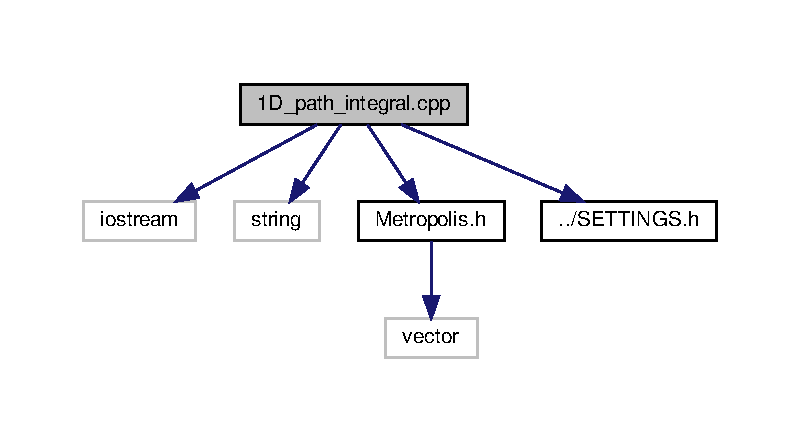
\includegraphics[width=350pt]{1D__path__integral_8cpp__incl}
\end{center}
\end{figure}


\subsection{Detailed Description}
Code to path integrate a 1D quantum system with Montecarlo method. 

In the main function, the physical parameters are set and the loop path integration is performed using the \hyperlink{classMetropolis}{Metropolis} algorithm, as implemented in the \hyperlink{classMetropolis}{Metropolis} class. Then, the requested observables are computed on the ensemble. Follow the comments in the source code of the \hyperlink{classMetropolis}{Metropolis} class for a more detailed description. 
\hypertarget{CUSTOM_8h}{}\section{C\+U\+S\+T\+O\+M.\+h File Reference}
\label{CUSTOM_8h}\index{C\+U\+S\+T\+O\+M.\+h@{C\+U\+S\+T\+O\+M.\+h}}


Header file to define the action of the system and the observables to be computed.  




\subsection{Detailed Description}
Header file to define the action of the system and the observables to be computed. 

Define here the implementation of the action in \hyperlink{classMetropolis_afb509c80a84817bf9b4ff183e02a44cb}{Metropolis\+::S}, that of the observable gamma in \hyperlink{classMetropolis_adf0ef3e12d4ce4185d3a536649de5cee}{Metropolis\+::\+Evaluate\+Gamma} and the one of the propagator in \hyperlink{classMetropolis_aa0e41567dcbb736f1bcc4a09dbb5f6fb}{Metropolis\+::\+Evaluate\+Propagator}. Please, follow the comments in the file for more specific indications. 
\hypertarget{Metropolis_8h}{}\section{Metropolis.\+h File Reference}
\label{Metropolis_8h}\index{Metropolis.\+h@{Metropolis.\+h}}


Header file for the definition of the class \hyperlink{classMetropolis}{Metropolis}.  


{\ttfamily \#include $<$vector$>$}\newline
Include dependency graph for Metropolis.\+h\+:
\nopagebreak
\begin{figure}[H]
\begin{center}
\leavevmode
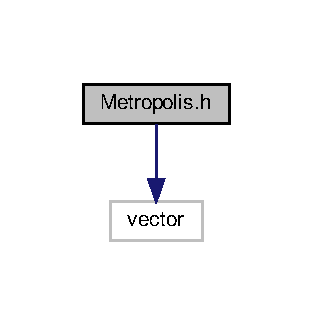
\includegraphics[width=150pt]{Metropolis_8h__incl}
\end{center}
\end{figure}
This graph shows which files directly or indirectly include this file\+:
\nopagebreak
\begin{figure}[H]
\begin{center}
\leavevmode
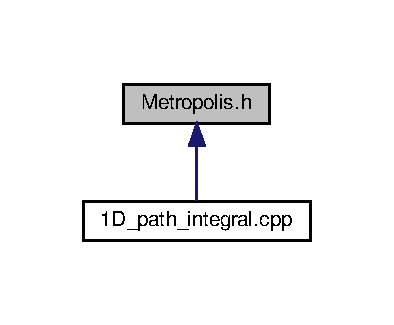
\includegraphics[width=189pt]{Metropolis_8h__dep__incl}
\end{center}
\end{figure}
\subsection*{Classes}
\begin{DoxyCompactItemize}
\item 
class \hyperlink{classMetropolis}{Metropolis}
\end{DoxyCompactItemize}


\subsection{Detailed Description}
Header file for the definition of the class \hyperlink{classMetropolis}{Metropolis}. 

Header file containing the definitions of the attributes and members of the class \hyperlink{classMetropolis}{Metropolis}. The instances of this class represent an implementation of the \hyperlink{classMetropolis}{Metropolis} algorithm for a physical quantum system in 1D via path integral formalism. The physical system is described by its euclidean action S, defined in the function \hyperlink{classMetropolis_afb509c80a84817bf9b4ff183e02a44cb}{Metropolis\+::S} and implemented in the \hyperlink{CUSTOM_8h}{C\+U\+S\+T\+O\+M.\+h} file. The observable Gamma, whose implementation is in the same \hyperlink{CUSTOM_8h}{C\+U\+S\+T\+O\+M.\+h} file, is estimated by averaging over the Montecarlo ensemble\+: the estimators for the chosen Gamma are readily provided by the method Metropolis\+::\+Compute\+Estimators. In addition, an estimate of the energy gap as a function of time can be obtained via \hyperlink{classMetropolis_a197d44f9109ce75781a70441f1d0b2b2}{Metropolis\+::\+Compute\+Energy\+Estimators} using the propagator defined in \hyperlink{CUSTOM_8h}{C\+U\+S\+T\+O\+M.\+h}\+: in this case, averages and standard deviations of the bootstrap copies of the Montecarlo ensemble are used. These separate implementations aim at providing flexibility both for choice of the physical system and that of the observable. Further comments may be found in the implementation file of this class. 
\hypertarget{plot__macro_8cpp}{}\section{plot\+\_\+macro.\+cpp File Reference}
\label{plot__macro_8cpp}\index{plot\+\_\+macro.\+cpp@{plot\+\_\+macro.\+cpp}}


R\+O\+OT macro to generate a plot from the \hyperlink{1D__path__integral_8cpp}{1\+D\+\_\+path\+\_\+integral.\+cpp} output.  


{\ttfamily \#include $<$algorithm$>$}\newline
{\ttfamily \#include $<$cmath$>$}\newline
{\ttfamily \#include $<$fstream$>$}\newline
{\ttfamily \#include $<$iostream$>$}\newline
{\ttfamily \#include $<$string$>$}\newline
{\ttfamily \#include \char`\"{}T\+Canvas.\+h\char`\"{}}\newline
{\ttfamily \#include \char`\"{}T\+F1.\+h\char`\"{}}\newline
{\ttfamily \#include \char`\"{}T\+Graph.\+h\char`\"{}}\newline
{\ttfamily \#include \char`\"{}T\+Graph\+Errors.\+h\char`\"{}}\newline
{\ttfamily \#include \char`\"{}S\+E\+T\+T\+I\+N\+G\+S.\+h\char`\"{}}\newline
Include dependency graph for plot\+\_\+macro.\+cpp\+:
\nopagebreak
\begin{figure}[H]
\begin{center}
\leavevmode
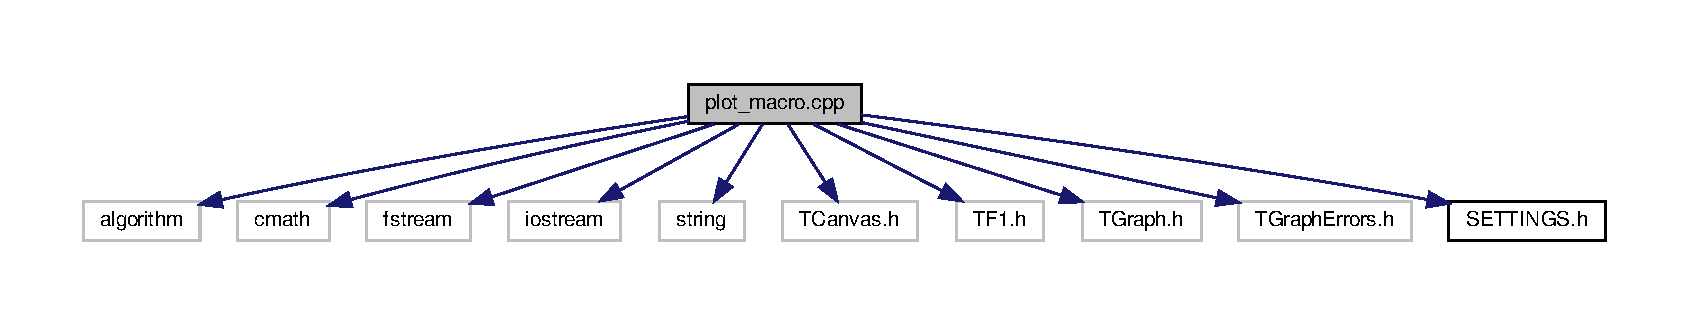
\includegraphics[width=350pt]{plot__macro_8cpp__incl}
\end{center}
\end{figure}


\subsection{Detailed Description}
R\+O\+OT macro to generate a plot from the \hyperlink{1D__path__integral_8cpp}{1\+D\+\_\+path\+\_\+integral.\+cpp} output. 

R\+O\+OT macro to generate a plot from the \hyperlink{1D__path__integral_8cpp}{1\+D\+\_\+path\+\_\+integral.\+cpp} output of the method \hyperlink{classMetropolis_a197d44f9109ce75781a70441f1d0b2b2}{Metropolis\+::\+Compute\+Energy\+Estimators}. Various graphical options are implemented and tuned in the code. Type\+:~\newline
 \$ R\+O\+OT \hyperlink{plot__macro_8cpp}{plot\+\_\+macro.\+cpp}~\newline
 to run and generate the plot \char`\"{}plot\+\_\+\+R\+O\+O\+T.\+png\char`\"{}. 
\hypertarget{plot__macro_8py}{}\section{plot\+\_\+macro.\+py File Reference}
\label{plot__macro_8py}\index{plot\+\_\+macro.\+py@{plot\+\_\+macro.\+py}}


Python code to generate a plot from the \hyperlink{1D__path__integral_8cpp}{1\+D\+\_\+path\+\_\+integral.\+cpp} output.  


\subsection*{Functions}
\begin{DoxyCompactItemize}
\item 
def \hyperlink{plot__macro_8py_ae039044acdd5795dee08952fc970d8e1}{plot\+\_\+macro.\+read\+\_\+param\+\_\+from\+\_\+file} (filename)
\begin{DoxyCompactList}\small\item\em Function to read parameters a, output\+\_\+name and N from header file. \end{DoxyCompactList}\end{DoxyCompactItemize}


\subsection{Detailed Description}
Python code to generate a plot from the \hyperlink{1D__path__integral_8cpp}{1\+D\+\_\+path\+\_\+integral.\+cpp} output. 

Python code to generate a plot from the \hyperlink{1D__path__integral_8cpp}{1\+D\+\_\+path\+\_\+integral.\+cpp} output of the method \hyperlink{classMetropolis_a197d44f9109ce75781a70441f1d0b2b2}{Metropolis\+::\+Compute\+Energy\+Estimators()}.Various graphical options are implemented and tuned in the code.\+Type \+:~\newline
\$ python \hyperlink{plot__macro_8py}{plot\+\_\+macro.\+py}~\newline
to run and generate the plot \char`\"{}plot\+\_\+py.\+png\char`\"{}. 

\subsection{Function Documentation}
\mbox{\Hypertarget{plot__macro_8py_file_ae039044acdd5795dee08952fc970d8e1}\label{plot__macro_8py_file_ae039044acdd5795dee08952fc970d8e1}} 
\index{plot\+\_\+macro.\+py@{plot\+\_\+macro.\+py}!read\+\_\+param\+\_\+from\+\_\+file@{read\+\_\+param\+\_\+from\+\_\+file}}
\index{read\+\_\+param\+\_\+from\+\_\+file@{read\+\_\+param\+\_\+from\+\_\+file}!plot\+\_\+macro.\+py@{plot\+\_\+macro.\+py}}
\subsubsection{\texorpdfstring{read\+\_\+param\+\_\+from\+\_\+file()}{read\_param\_from\_file()}}
{\footnotesize\ttfamily def plot\+\_\+macro.\+read\+\_\+param\+\_\+from\+\_\+file (\begin{DoxyParamCaption}\item[{}]{filename }\end{DoxyParamCaption})}



Function to read parameters a, output\+\_\+name and N from header file. 


\begin{DoxyParams}{Parameters}
{\em filename} & name of the header file to look into. \\
\hline
\end{DoxyParams}
\begin{DoxySeeAlso}{See also}
\hyperlink{SETTINGS_8h}{S\+E\+T\+T\+I\+N\+G\+S.\+h} 
\end{DoxySeeAlso}

\hypertarget{SETTINGS_8h}{}\section{S\+E\+T\+T\+I\+N\+G\+S.\+h File Reference}
\label{SETTINGS_8h}\index{S\+E\+T\+T\+I\+N\+G\+S.\+h@{S\+E\+T\+T\+I\+N\+G\+S.\+h}}


Header file to set the adjustable parameters of the system.  


This graph shows which files directly or indirectly include this file\+:
\nopagebreak
\begin{figure}[H]
\begin{center}
\leavevmode
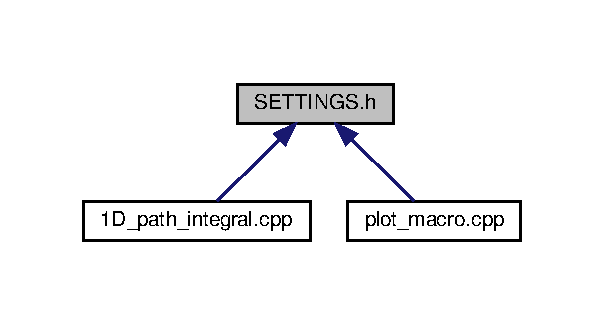
\includegraphics[width=290pt]{SETTINGS_8h__dep__incl}
\end{center}
\end{figure}
\subsection*{Variables}
\begin{DoxyCompactItemize}
\item 
\mbox{\Hypertarget{SETTINGS_8h_a7722c8ecbb62d99aee7ce68b1752f337}\label{SETTINGS_8h_a7722c8ecbb62d99aee7ce68b1752f337}} 
int \hyperlink{SETTINGS_8h_a7722c8ecbb62d99aee7ce68b1752f337}{N} = 20
\begin{DoxyCompactList}\small\item\em Number of sites. \end{DoxyCompactList}\item 
\mbox{\Hypertarget{SETTINGS_8h_a12bee834e3763c6d1de9a130cd451aed}\label{SETTINGS_8h_a12bee834e3763c6d1de9a130cd451aed}} 
int \hyperlink{SETTINGS_8h_a12bee834e3763c6d1de9a130cd451aed}{Ncorr} = 20
\begin{DoxyCompactList}\small\item\em Number of correlated path configurations to skip before next acquisition. \end{DoxyCompactList}\item 
\mbox{\Hypertarget{SETTINGS_8h_aec02ce37912e1f500d7eb7fb3c8b6e1f}\label{SETTINGS_8h_aec02ce37912e1f500d7eb7fb3c8b6e1f}} 
int \hyperlink{SETTINGS_8h_aec02ce37912e1f500d7eb7fb3c8b6e1f}{Ncf} = 10000
\begin{DoxyCompactList}\small\item\em Total number of path configurations to be sampled. \end{DoxyCompactList}\item 
\mbox{\Hypertarget{SETTINGS_8h_a71e3c918b5180d769d66c9f9868db86b}\label{SETTINGS_8h_a71e3c918b5180d769d66c9f9868db86b}} 
int \hyperlink{SETTINGS_8h_a71e3c918b5180d769d66c9f9868db86b}{N\+Boot\+Straps} = 100
\begin{DoxyCompactList}\small\item\em Number of bootstraps to perform on the Ncf configurations. \end{DoxyCompactList}\item 
\mbox{\Hypertarget{SETTINGS_8h_a4904cc82627458fdf6672ccc0b2802c7}\label{SETTINGS_8h_a4904cc82627458fdf6672ccc0b2802c7}} 
double \hyperlink{SETTINGS_8h_a4904cc82627458fdf6672ccc0b2802c7}{epsilon} = 1.\+4
\begin{DoxyCompactList}\small\item\em Typical magnitude of a path update. \end{DoxyCompactList}\item 
\mbox{\Hypertarget{SETTINGS_8h_a1031d0e0a97a340abfe0a6ab9e831045}\label{SETTINGS_8h_a1031d0e0a97a340abfe0a6ab9e831045}} 
double \hyperlink{SETTINGS_8h_a1031d0e0a97a340abfe0a6ab9e831045}{a} = 0.\+5
\begin{DoxyCompactList}\small\item\em Time discretization, i.\+e. grid spacing. \end{DoxyCompactList}\item 
\mbox{\Hypertarget{SETTINGS_8h_a4bfaa4b497cb5e62d0cfc56f5ce8cfc9}\label{SETTINGS_8h_a4bfaa4b497cb5e62d0cfc56f5ce8cfc9}} 
std\+::string \hyperlink{SETTINGS_8h_a4bfaa4b497cb5e62d0cfc56f5ce8cfc9}{output\+\_\+name} = \char`\"{}Ncf\+\_\+10000\+\_\+100\+B.\+dat\char`\"{}
\begin{DoxyCompactList}\small\item\em Output filename (relative to this directory) \end{DoxyCompactList}\end{DoxyCompactItemize}


\subsection{Detailed Description}
Header file to set the adjustable parameters of the system. 

Set here the parameters of the system, namely\+: the number of sites N, the number of correlated path configurations to skip Ncorr, the number of path configurations to be sampled Ncf, the number of bootstrap copies N\+Boot\+Straps, the magnitude of a path update epsilon, the time spacing a and the output filename output\+\_\+name. If you wish to run the \hyperlink{classMetropolis_aa733da324aa14e6c2fcf9c75f5643cbe}{Metropolis\+::\+Compute\+Binned\+Energy\+Estimators} method, make sure to define also the integer for the bin size. 
%--- End generated contents ---

% Index
\backmatter
\newpage
\phantomsection
\clearemptydoublepage
\addcontentsline{toc}{chapter}{Index}
\printindex

\end{document}
